\section{ \bfseries Equality Constrained Convex QP}

\begin{align*}
&\min_{x} \quad \phi=\frac{1}{2} x^{\prime} H x+g^{\prime} x \tag{1}\label{con:op1}\\
& s.t. \quad A^{\prime} x=b\\
&\text{with}\quad H \succ 0
\end{align*}



%%%%%%%%%%%%%%%%%%%%%%%%%%%%%%%%%%%%%%%%%%
%%%%%%%%%%%%%%%%%%%%%%%%%%%%%%%%%%%%%%%%%%%%%%%%%%%%%%%%%%%%%%%%%%%%%%%%%%%%%%%%%%%%%
%%%%%%%%%%%%%%%%%%%%%%%%%%%%%%%%%%%%%%%%%%%
%%%%%%%%%%%%%%%%%%%%%%%%%%%%%%%%%%%%%%%%%%
%%%%%%%%%%%%%%%%%%%%%%%%%%%%%%%%%%%%%%%%%%%
\subsection{\bfseries Lagrangian function}
\definecolor{shadecolor}{rgb}{0.92,0.92,0.92}
\begin{shaded}
{ Question: What is the Lagrangian function for this problem?}
\end{shaded}
\begin{align*}
L(x, \lambda)&=f(x)-\sum_{i \in \mathcal{E}} \lambda_{i} c_{i}(x)\\
&=\frac{1}{2} x^{\prime} H x+g^{\prime} x-\lambda^{\prime}(A^{\prime}x-b)
\end{align*}




%%%%%%%%%%%%%%%%%%%%%%%%%%%%%%%%%%%%%%%%%%
%%%%%%%%%%%%%%%%%%%%%%%%%%%%%%%%%%%%%%%%%%%
%%%%%%%%%%%%%%%%%%%%%%%%%%%%%%%%%%%%%%%%%%
%%%%%%%%%%%%%%%%%%%%%%%%%%%%%%%%%%%%%%%%%%%
%%%%%%%%%%%%%%%%%%%%%%%%%%%%%%%%%%%%%%%%%%
%%%%%%%%%%%%%%%%%%%%%%%%%%%%%%%%%%%%%%%%%%%
\subsection{\bfseries Optimality conditions}
\begin{shaded}
{Question: What is the first order necessary optimality conditions for this problem? Are they
also sufficient and why?}
\end{shaded}
\bm{$Theorem\ (Necessary\ 1st\  Order\  Conditions)$}\\
Let x be a local minimizer of (\ref{con:op1}). Then
\begin{flalign}
&\ 1.\ \nabla_{x} L\left(x,\lambda\right)=Hx+g-A\lambda=0&\\
&\ 2.\ c_{i}\left(x\right)=A^{\prime}x-b=0 \quad i \in \mathcal{E}&
\end{flalign}
The constrained optimization problem (\ref{con:op1}) is convex because\\[0.3cm]
\ 1.\ $\phi$ is convex\ (H is positive definite).\\
\ 2.\ The equality constraints are linear.\\[0.3cm]
So the first order optimality conditions are sufficient for this problem. 




%%%%%%%%%%%%%%%%%%%%%%%%%%%%%%%%%%%%%%%%%%
%%%%%%%%%%%%%%%%%%%%%%%%%%%%%%%%%%%%%%%%%%%%%%%%%%%%%%%%%%%%%%%%%%%%%%%%%%%%%%%%%%%%%
%%%%%%%%%%%%%%%%%%%%%%%%%%%%%%%%%%%%%%%%%%%
%%%%%%%%%%%%%%%%%%%%%%%%%%%%%%%%%%%%%%%%%%
%%%%%%%%%%%%%%%%%%%%%%%%%%%%%%%%%%%%%%%%%%%
\newpage
\subsection{\bfseries Solvers implementation}
\begin{shaded}
{Question: Implement solvers for solution of the problem (1.1) that are based on an LU-factorization (dense), LU-factorization (sparse), LDL-factorization (dense), LDL-factorization (sparse), a range-space factorization, and a null-space factorization.
You must provide pseudo-code and source code for your implementation.}
\end{shaded}
Through the the first order optimality conditions listed, The convex equality constrained QP is solved by solution of the
KKT system\\
$$\overbrace{\begin{bmatrix}
H & -A\\
-A^{\prime} & 0
\end{bmatrix}}^{=KKT_{A}}
\overbrace{
\begin{bmatrix}
x\\
\lambda
\end{bmatrix}}^{=z}=
\overbrace{
-\begin{bmatrix}
g\\
b
\end{bmatrix}}^{=KKT_b}\eqno{(1.3)}$$\\[0.3cm]
Then the methods to factorize the KKT system are discussed. Please find the interface function "EqualityQPSolver" which can switch between the different solvers in the Appendix section \ref{6.1.1}.





%%%%%%%%%%%%%%%%%%%%%%%%%%%%%%%%%%%%%%%%%%
%%%%%%%%%%%%%%%%%%%%%%%%%%%%%%%%%%%%%%%%%%%
\subsubsection{\bfseries LU factorization (dense)}
Assuming that the $KKT_A$ is a square and nonsingular matrix. The LU factorization can be used with partial pivoting to decompose the matrix $KKT_A$ into an upper triangular matrix U, a lower triangular matrix L, and a permutation matrix P such that\\
$$PA=LU$$
Then backward and forward substitution can be performed with the triangular factors. But this method has the disadvantage that it ignores the symmetry. In the implementation, LU-factorization returns the row permutations p as a vector instead of a matrix P in order to save the memory. 

{\setmainfont{Courier New Bold} \scriptsize        
\begin{lstlisting}
function [x,lambda]=EqualityQPSolverLUdense(H,g,A,b)
%EqualityQPSolverLUdense  Equality constrained convex QP
%Syntax: [x,lambda]=EqualityQPSolverLUdense(H,g,A,b)

%dimension of A>>>>>number of x and equality constraints
[nx,nc]=size(A);
%setup KKT system(dense)
KKT_A=[H -A;-A' zeros(nc,nc)];
KKT_b=-[g;b];
% factorize and solve KKT system using the LU factorization
[L,U,p]=lu(KKT_A,'vector');
z=U\(L\KKT_b(p));
%Extract solution
x=z(1:nx);
lambda=z(nx+1:end);
end
\end{lstlisting}}

%%%%%%%%%%%%%%%%%%%%%%%%%%%%%%%%%%%%%%%%%%
%%%%%%%%%%%%%%%%%%%%%%%%%%%%%%%%%%%%%%%%%%%
\subsubsection{\bfseries LU factorization (sparse)}
Compared with the LU factorization(dense), The KKT matrix is represented as a sparse matrix.

{\setmainfont{Courier New Bold}      \scriptsize       
\begin{lstlisting}
function [x,lambda]=EqualityQPSolverLUsparse(H,g,A,b)
%EqualityQPSolverLUsparse Equality constrained convex QP

%Syntax: [x,lambda]=EqualityQPSolverLUsparse(H,g,A,b)

%dimension of A>>>>>>number of x and equality constraints
[nx,nc]=size(A);
%setup KKT system(dense)
KKT_A=[H -A;-A' zeros(nc,nc)];
KKT_b=-[g;b];
%sparse KKT system
KKT_A=sparse(KKT_A);
KKT_b=sparse(KKT_b);
% factorize and solve KKT system using the LU factorization
[L,U,p]=lu(KKT_A,'vector');% factorization
z=U\(L\KKT_b(p));% back substitution
%Extract solution
x=z(1:nx);
lambda=z(nx+1:end);
end
\end{lstlisting}}



%%%%%%%%%%%%%%%%%%%%%%%%%%%%%%%%%%%%%%%%%%
%%%%%%%%%%%%%%%%%%%%%%%%%%%%%%%%%%%%%%%%%%%
\subsubsection{\bfseries LDL factorization (dense)}
For a symmetric positive definite matrix $KKT_A$, the factorization has the form
$$P^{\prime}(KKT_A)P=LBL^{\prime}\eqno{(1.4)}$$
where P is the permutation matrix, L is the lower triangular matrix and B is a block diagonal
matrix. The symmetric permutation defined by the matrix P are introduced for numerical sability of the computation.

{\setmainfont{Courier New Bold}  \scriptsize           
\begin{lstlisting}
function [x,lambda]=EqualityQPSolverLDLdense(H,g,A,b)
%EqualityQPSolverLDLdense  Equality constrained convex QP

%Syntax: [x,lambda]=EqualityQPSolverLDLdense(H,g,A,b)

%dimension of A>>>>>>>number of x and equality constraints
[nx,nc]=size(A);
%setup KKT system(dense)
KKT_A=[H -A;-A' zeros(nc,nc)];
KKT_b=-[g;b];
% factorize and solve KKT system using the LDL factorization
z=zeros(nx+nc,1);
[L,D,p]=ldl(KKT_A,'vector');% factorization
z(p)=L'\(D\(L\KKT_b(p)));% back substitution
%Extract solution
x=z(1:nx);
lambda=z(nx+1:end);
end
\end{lstlisting}}



%%%%%%%%%%%%%%%%%%%%%%%%%%%%%%%%%%%%%%%%%%
%%%%%%%%%%%%%%%%%%%%%%%%%%%%%%%%%%%%%%%%%%%
\subsubsection{\bfseries LDL factorization (sparse)}
Compared with the LDL factorization(dense), The KKT matrix is represented as a sparse matrix

{\setmainfont{Courier New Bold}   \scriptsize          
\begin{lstlisting}
function [x,lambda]=EqualityQPSolverLDLsparse(H,g,A,b)
%EqualityQPSolverLDLsparse  Equality constrained convex QP

%Syntax: [x,lambda]=EqualityQPSolverLDLsparse(H,g,A,b)

%dimension of A------>number of x and equality constraints
[nx,nc]=size(A);
%setup KKT system(dense)
KKT_A=[H -A;-A' zeros(nc,nc)];
KKT_b=-[g;b];
%sparse KKT system
KKT_A=sparse(KKT_A);
KKT_b=sparse(KKT_b);
% factorize and solve KKT system using the LDL factorization
z=zeros(nx+nc,1);
[L,D,p]=ldl(KKT_A,'vector');% factorization
z(p)=L'\(D\(L\KKT_b(p)));% back substitution
%Extract solution
x=z(1:nx);
lambda=z(nx+1:end);
end
\end{lstlisting}}



%%%%%%%%%%%%%%%%%%%%%%%%%%%%%%%%%%%%%%%%%%
%%%%%%%%%%%%%%%%%%%%%%%%%%%%%%%%%%%%%%%%%%%
\subsubsection{\bfseries Range-Space factorization}
Assume that the KKT system\\
$$\begin{bmatrix}
H & -A\\
-A^{\prime} & 0
\end{bmatrix}
\begin{bmatrix}
x\\
\lambda
\end{bmatrix}=
-\begin{bmatrix}
g\\
b
\end{bmatrix} \quad A \in \mathbb{R}^{n \times m}$$\\[0.3cm]
The Range-Space method is useful when\\
1.$H$ is well-conditioned and easy to invert ($H$ is diagonal or block-diagonal).\\
2.$H^{\prime}$ is known explicitly.\\
3.The number of equality constraints (m) is small.\\[0.3cm]
From the KKT system
$$Hx-A\lambda=-g \quad \Leftrightarrow \quad x=H^{-1}A\lambda-H^{-1}g$$
Substitute it into second equation
\begin{align*}
b=A^{\prime}x&=\left(A^{\prime}H^{-1}A\right)\lambda-A^{\prime}H^{-1}g\\
\lambda&=\left(A^{\prime}H^{-1}A\right)^{-1}\left(b+A^{\prime}H^{-1}g\right)
\end{align*}\\[0.3cm]
{\setmainfont{Times New Roman}\bfseries Pseudo-code}
\begin{algorithm}[!h]
	\caption{Range-Space factorization}
	\begin{algorithmic}[1]
		\STATE Cholesky factorize $H = LL^{\prime}$
		\STATE Solve $Hv = g$ for $v$
		\STATE Form $H_A = A^{\prime}H^{-1}A = L_AL_A^{\prime}$ and its factorization
		\STATE Solve $H_A\lambda = b + A^{\prime}v$ for $\lambda$
		\STATE Solve $Hx = A\lambda - g$ for $x$
	\end{algorithmic}
\end{algorithm}

{\setmainfont{Courier New Bold} \scriptsize            
\begin{lstlisting}
function [x,lambda]=EqualityQPSolverRangeSpace(H,g,A,b)
%EqualityQPSolverRangeSpace  Equality constrained convex QP

%Syntax: [x,lambda]=EqualityQPSolverRangeSpace(H,g,A,b)
%H is positive definite

%solve Hv=g
v=H\g;
%form HA
H_A=A'*inv(H)*A;
%solve lambda
lambda=H_A\(b+A'*v);
%solve x
x=H\(A*lambda-g);
end
\end{lstlisting}}



%%%%%%%%%%%%%%%%%%%%%%%%%%%%%%%%%%%%%%%%%%
%%%%%%%%%%%%%%%%%%%%%%%%%%%%%%%%%%%%%%%%%%%
\subsubsection{\bfseries Null-Space factorization}
Assume that the KKT system\\
$$\begin{bmatrix}
H & -A\\
-A^{\prime} & 0
\end{bmatrix}
\begin{bmatrix}
x\\
\lambda
\end{bmatrix}=
-\begin{bmatrix}
g\\
b
\end{bmatrix} \quad A \in \mathbb{R}^{n \times m}$$\\[0.3cm]
The Null-Space method is useful when the number of degrees of freedom, $n- m$, is small. But The Null-Space method does not require nonsingularity of $H$ and therefore has wider applicability than the Range-Space method.\\[0.3cm]
The non-singular matrix $[Y \quad Z]\in \mathbb{R}^{n \times n}$with $Y\in \mathbb{R}^{n \times m}$\ and\ $Z\in \mathbb{R}^{n \times (n-m)}$ is defined such that
\begin{align*}
A^{\prime}[Y \quad Z]&=\left[
A^{\prime} Y \quad A^{\prime} Z\right]
=\left[A^{\prime} Y \quad 0\right] \quad A^{\prime} Y \in \mathbb{R}^{m \times m}\text { non-singular }\\
x&=Yx_Y+Zx_Z \tag{1.5}\label{1.5}
\end{align*}
Substitute equation (\ref{1.5}) into the second equation of KKT system
$$b=A^{\prime}x=A^{\prime}Yx_y+A^{\prime}Zx_Z=A^{\prime}Yx_Y\eqno{(1.6)}$$
Substitute equation (\ref{1.5}) into the first equation of KKT system
\begin{align*}
-g&=Hx-A\lambda\\
\left(A^{\prime}Y\right)^{\prime}\lambda&=Y^{\prime}\left(Hx+g\right)\tag{1.7}
\end{align*}
\begin{align*}
-g=Hx-A\lambda&=HYx_Y+HZx_Z-A\lambda\\
\left(Z^{\prime}HZ\right)x_Z&=-Z^{\prime}\left(HYx_Y+g\right)+Z^{\prime}A\lambda\\
\left(Z^{\prime}HZ\right)x_Z&=-Z^{\prime}\left(HYx_Y+g\right)\tag{1.8}
\end{align*}
The Null-Space method implemented is based on the QR-Factorization
$$A=Q\begin{bmatrix}
R\\0
\end{bmatrix}=\left[Q1 \quad Q2\right]\begin{bmatrix}
R\\0
\end{bmatrix}=Q1R$$
$$\left[Y \quad Z\right]=\left[Q1 \quad Q2\right] \quad A^{\prime}Y=A^{\prime}Q1=R^{\prime}$$
Where Q2 is our null space.\\[0.3cm]

{\setmainfont{Times New Roman}\bfseries Pseudo-code}
\begin{algorithm}[!h]
	\caption{Null-Space factorization}
	\begin{algorithmic}[1]
	    \STATE QR factorization of $A \in \mathbb{R}^{n \times m}$
		\STATE Solve $R^{\prime}x_Y=b$
		\STATE Solve $\left(Q2^{\prime}HQ2\right)x_Z=-Q2^{\prime}\left(HQ1x_Y+g\right)$
		\STATE Compute $x=Q1x_Y+Q2x_Z$
		\STATE Solve $R\lambda=Q1^{\prime}\left(Hx+g\right)$
	\end{algorithmic}
\end{algorithm}


{\setmainfont{Courier New Bold} \scriptsize            
\begin{lstlisting}
function [x,lambda]=EqualityQPSolverNullSpace(H,g,A,b)
%EqualityQPSolverNullSpace  Equality constrained convex QP

%Syntax: [x,lambda]=EqualityQPSolverNullSpace(H,g,A,b)

%dimension of A>>>>>>>>number of x and equality constraints
[nx,nc]=size(A);
%QR factorization
[Q,Rbar] = qr(A);
m1 = size(Rbar,2);
Q1 = Q(:,1:m1); 
Q2 = Q(:,m1+1:nx);
R = Rbar(1:m1,1:m1);

xY=R'\b;
xZ=(Q2'*H*Q2)\(-Q2'*(H*Q1*xY+g));
x=Q1*xY+Q2*xZ;
lambda=R\(Q1'*(H*x+g));
end
\end{lstlisting}}

%%%%%%%%%%%%%%%%%%%%%%%%%%%%%%%%%%%%%%%%%%
%%%%%%%%%%%%%%%%%%%%%%%%%%%%%%%%%%%%%%%%%%%%%%%%%%%%%%%%%%%%%%%%%%%%%%%%%%%%%%%%%%%%%
%%%%%%%%%%%%%%%%%%%%%%%%%%%%%%%%%%%%%%%%%%%%%%%%%%%%%%%%%%%%%%%%%%%%%%%%%%%%%%%%%%%%%
%%%%%%%%%%%%%%%%%%%%%%%%%%%%%%%%%%%%%%%%%%%

\newpage
\subsection{\bfseries Implementation test}
\begin{shaded}
{Question: Test your implementation on a size dependent problem structure and report the
results. You are free to chose the problems that you want to use for testing your
algorithm.}
\end{shaded}
%%%%%%%%%%%%%%%%%%%%%%%%%%%%%%%%%%%%%%%%
%%%%%%%%%%%%%%%%%%%%%%%%%%%%%%%%%%%%%%%%%%%
\subsubsection{\bfseries Problem description}
The first question of Exercise 5 provided by the teacher will be selected to test the implemented solvers. Consider the convex quadratic optimization problem\\
\begin{align*}
&\min_{u} \quad \sum_{i=1}^{n+1} \left(u_i-\bar{u}\right)^2 \tag{1.9}\\
& s.t. \quad -u_1+u_n=-d0\\
& \quad \quad \ u_i-u_{i+1}=0 \qquad \qquad i=1,2,...n-2\\
& \quad \quad \ u_{n-1}-u_n-u_{n+1}=0
\end{align*}
$\bar{u}$ and $d_0$ are parameters of the problem. The problem size can be adjusted selecting
$n \ge 3$. Let $\bar{u} = 0.2$ and $d_0 = 1$. \\
A matlab function that constructs $H$,$g$,$A$, and $b$ as function of $n$, $\bar{u}$, and $d_0$ is implemented. Please see the function in the Appendix, section \ref{6.1.2}.
\subsubsection{\bfseries Result}
The first test carried out about the CPU time of LU-factorization (dense),  LDL-factorization (dense),  a range-space factorization, and a null-space factorization between 10 and 1000 variables. The matlab code of test is showed in Appendix section \ref{6.1.3}.\\
The curve of CPU time of these four methods is showed
\begin{figure}[H]
\centering
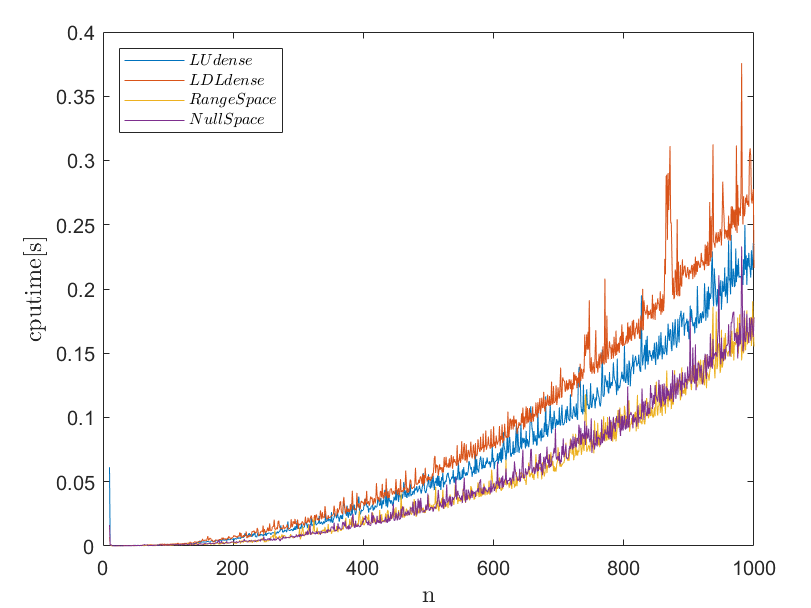
\includegraphics[scale=0.7]{figures/EQ_NOSPARSE.PNG}
\caption{CPU time of LU-dense, LDL-dense, range-space, and null-space}
\label{fig:labe1.4.1}
\end{figure}
It is found that with the increase in the number of variables, the CPU time required by the four factorization is gradually increasing. Compared with LU-factorization (dense) and LDL-factorization (dense), range-space factorization and null-space factorization take less CPU time and maintain almost the same performance. LU and LDL require the same CPU time when the number of variables is small, but as the number of variables increases, the difference between the CPU time required for LDL and LU gradually increases.\\
Then the CPU time of LU-factorization (sparse) and LDL-factorization (sparse) is test. The curve of CPU time of these LU-dense, LU-sparse, LDL-dense and LDL-sparse is showed
\begin{figure}[H]
\centering
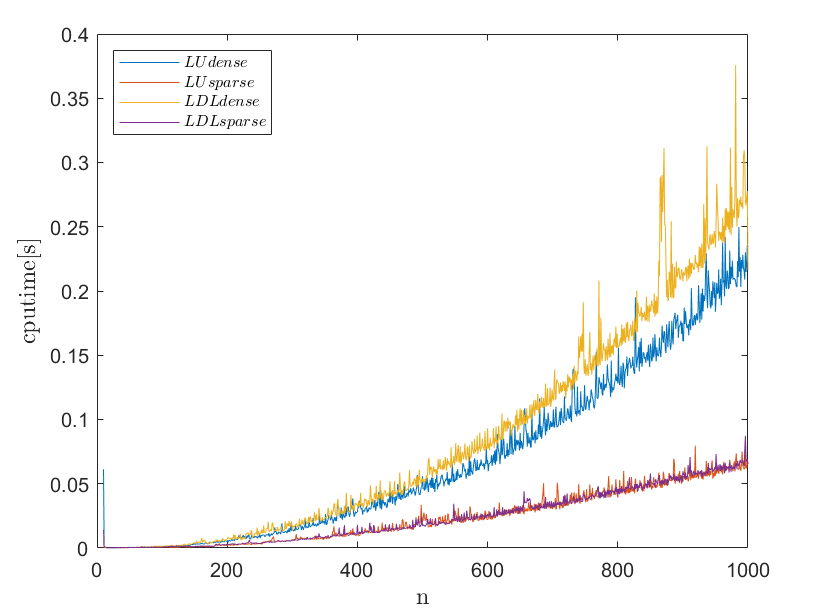
\includegraphics[scale=0.7]{figures/EQ_KKT_LULDL.PNG}
\caption{CPU time of LU-dense, LU-sparse, LDL-dense and LDL-sparse}
\label{fig:labe1.4.2}
\end{figure}
It is found that both the sparse factorization of LU and LDL significantly reduce CPU time compared to their respective dense factorization, and maintain similar performance.\\
The CPU time curves of all methods are shown here
\begin{figure}[H]
\centering
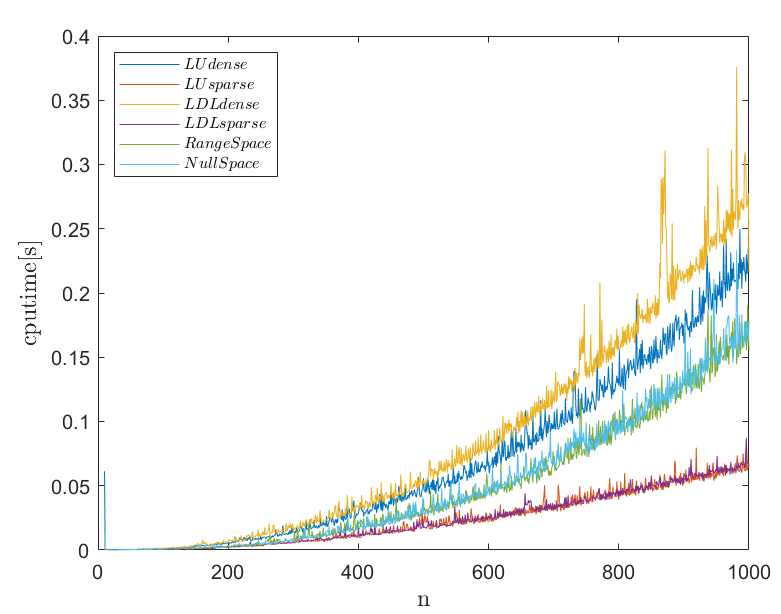
\includegraphics[scale=0.7]{figures/EQ_ALL.PNG}
\caption{CPU time of LU-dense, LU-sparse, LDL-dense, LDL-sparse, range-space, and null-space}
\label{fig:labe1.4.3}
\end{figure}
It can be seen that the sparse method factorization LDL and LU requires the least CPU time, and can maintain a CPU time of less than 0.1s when the KKT matrix is $1000 \times 1000$, while range-space factorization and null-space factorization need to be less than about 0.2s, and the dense factorization of LU requires less than 0.25s, and the dense factorization of LDL takes the most CPU time, which takes about 0.3s.